% ====================================================================
% VİZE RAPOR ŞABLONU – Türk Masalları Derlemesi Web Sayfası
% --------------------------------------------------------------------
% DERLEME: Overleaf'te Menu > Compiler > XeLaTeX (pdfLaTeX de çalışır).
%
% KURALLAR (şablonu kullanmadan önce okuyun):
%  1. Bölüm başlıklarını SİLMEYİN ve sırasını DEĞİŞTİRMEYİN.
%  2. [KÖŞELİ PARANTEZ] içindeki ve gri renkli açıklama metinlerini
%     kendi bilgilerinizle değiştirin; açıklama metinlerini silin.
%  3. MEBİS'e YALNIZCA bu raporun PDF'ini yükleyin.
%     ZIP ve HTML dosyası YÜKLEMEYİN. Tüm kontroller GitHub'dan yapılır.
%  4. Kapaktaki GitHub ve YouTube bağlantıları doğru ve tıklanabilir
%     olmalıdır. Teslimden önce PDF'teki bağlantılara tıklayıp deneyin.
%  5. Haftalık katkı tablosundaki görseller için resim dosyalarını
%     (hafta1.png, hafta2.png, ...) Overleaf projesine yükleyin.
%     Dosya adlarında boşluk ve Türkçe karakter kullanmayın.
%     Resim yoksa tabloda "görsel ekleyin" kutusu görünür.
%  6. Yapay zekâ kullandıysanız Bölüm 5'i doldurun.
% ====================================================================
\documentclass[12pt,a4paper]{article}

\usepackage{iftex}
\ifPDFTeX
  \usepackage[T1]{fontenc}
  \usepackage[utf8]{inputenc}
\else
  \usepackage{fontspec}
\fi
\usepackage[turkish]{babel}
\usepackage[margin=2.4cm]{geometry}
\usepackage{setspace}
\usepackage{graphicx}
\usepackage{float}
\usepackage{booktabs}
\usepackage{longtable}
\usepackage{array}
\usepackage{colortbl}
\usepackage{xcolor}
\usepackage{enumitem}
\usepackage{listings}
\usepackage{amssymb}
\usepackage{caption}
\usepackage{fancyhdr}
\usepackage{hyperref}

\onehalfspacing
\setlength{\parindent}{0pt}
\setlength{\parskip}{6pt}
\setlist{itemsep=2pt, topsep=4pt}
\hypersetup{colorlinks=true, linkcolor=blue!50!black, urlcolor=blue!50!black}

\definecolor{ana}{HTML}{14325C}
\definecolor{acik}{HTML}{EEF2F8}

\lstset{basicstyle=\ttfamily\small, backgroundcolor=\color{acik},
  frame=single, rulecolor=\color{ana}, breaklines=true,
  columns=fullflexible, keepspaces=true, showstringspaces=false}

\pagestyle{fancy}
\fancyhf{}
\fancyhead[L]{MASAL ATLASI}
\fancyhead[R]{Vize Raporu}
\fancyfoot[C]{\thepage}

% ---------- Yardımcı komutlar ----------
% Gri açıklama metni (silinecek yönergeler için)
\newcommand{\aciklama}[1]{{\color{gray}\itshape (#1)}}

% Haftalık tablo görseli: dosya yoksa "görsel ekleyin" kutusu çıkar
\newcommand{\haftagorsel}[1]{%
  \IfFileExists{#1}{%
    \includegraphics[width=\linewidth,height=4.2cm,keepaspectratio]{#1}%
  }{%
    \fbox{\parbox[c][2.6cm][c]{\dimexpr\linewidth-2\fboxsep-2\fboxrule\relax}{%
      \centering\small\color{gray} Ekran görüntüsü / görsel ekleyin\\ \texttt{#1}}}%
  }%
}
% Haftalık katılım kutuları (işaretlemek için $\square$ yerine $\boxtimes$ yazın)
\newcommand{\katilimkutulari}{\par\vspace{3pt}\small $\square$ Ders içinde katılım sergiledim\par $\square$ Telafi yaptım}

% Ek görsel: dosya yoksa hiçbir şey göstermez
\newcommand{\haftaek}[1]{%
  \IfFileExists{#1}{\\[4pt]\includegraphics[width=\linewidth,height=4.2cm,keepaspectratio]{#1}}{}%
}

% ---------- Kapak bilgileri ----------
\newcommand{\universite}{[İstanbul Medipol Üniversitesi / Görsel İletişim Tasarımı]}
\newcommand{\dersadi}{[Programlamaya Giriş]}
\newcommand{\hocaadi}{[Meral Şentürk]}
\newcommand{\ogrenciadi}{[Latife Beyza Yılmaz]}
\newcommand{\ogrencino}{[86230016]}
\newcommand{\projeadi}{MASAL ATLASI}
% Bağlantıları tam adres olarak yazın (https:// ile başlayarak)
\newcommand{\githublink}{\url{https://github.com/latifebeyzayilmaz9/Masal-Atlas-}}
\newcommand{\youtubelink}{\url{https://youtu.be/0LZKcCXk2jo}}

\begin{document}

% ====================================================================
% KAPAK
% ====================================================================
\begin{titlepage}
\centering
\vspace*{1cm}
{\large \universite \par}
\vspace{1.8cm}
{\Huge\bfseries\color{ana} \projeadi \par}
\vspace{0.4cm}
{\Large Türk Masalları Derlemesi Web Sayfası \par}
{\large Vize Raporu \par}
\vspace{1.8cm}
{\large \textbf{Ders:} \dersadi \par}
{\large \textbf{Öğretim Üyesi:} \hocaadi \par}
\vspace{1.2cm}
{\large \textbf{Hazırlayan:} \ogrenciadi \par}
{\large \textbf{Öğrenci No:} \ogrencino \par}
\vspace{1.8cm}
\fbox{\parbox{0.88\linewidth}{\centering\vspace{6pt}
{\large\bfseries Proje Bağlantıları}\\[8pt]
\textbf{GitHub deposu:}\\ \githublink \\[8pt]
\textbf{YouTube sunum videosu:}\\ \youtubelink
\vspace{6pt}}}
\vfill
{\large \today \par}
\end{titlepage}

\tableofcontents
\newpage

% ====================================================================
\section{Giriş}
% ====================================================================
Masal Atlası, Türk masallarını dijital ortamda bir araya getirerek geleneksel anlatı kültürünü görsel ve etkileşimli bir deneyimle sunmayı amaçlayan bir web sayfası projesidir. Projenin temel amacı, kültürel mirasımızın önemli bir parçası olan masalları kullanıcıların kolayca keşfedebileceği ve okuyabileceği bir platform oluşturmaktır. Tasarım sürecinde Türk minyatür sanatından ve geleneksel kitap süslemelerinden ilham alınarak masalların atmosferini destekleyen bir görsel dil oluşturulmuştur. Web sayfasında farklı anlatı özelliklerine sahip toplam 12 Türk masalına yer verilmiş ve her masal kendine özgü bir illüstrasyonla desteklenmiştir. Proje, HTML kullanılarak yapılandırılmış; görsel düzenlemeler içsel CSS, kullanıcı etkileşimleri ise içsel JavaScript ile gerçekleştirilmiştir. Masal arama, masallar arasında gezinme ve yazı boyutunu değiştirme gibi özellikler sayesinde kullanıcıların okuma deneyimini kişiselleştirmesi hedeflenmiştir. Tüm içerikler tek bir HTML dosyasında birleştirilerek web sayfasının internet bağlantısı olmadan da çalışması sağlanmış ve farklı ekran boyutlarında kullanılabilirliği test edilmiştir. Bu raporda projenin tasarım kararları, teknik geliştirme süreci, kullanılan araçlar ve test sonuçları ele alınmaktadır.

\subsection{Proje Özeti}
Masal Atlası, 12 Türk masalını özgün illüstrasyonlarla bir araya getiren, kullanıcıların masalları arayabildiği ve okuyabildiği etkileşimli bir web sayfasıdır. Geleneksel Türk minyatür sanatından esinlenen görsel tasarımı, sade gezinme yapısı ve kişiselleştirilebilir okuma özellikleriyle kültürel anlatıları dijital ortamda erişilebilir kılmayı amaçlamaktadır. Proje, HTML, CSS ve JavaScript kullanılarak tek dosya hâlinde geliştirilmiş ve çevrimdışı çalışacak şekilde düzenlenmiştir.

\subsection{Gereksinimlerin Karşılanması}
\begin{center}
\rowcolors{2}{acik}{white}
\begin{tabular}{@{}p{8.2cm}c@{}}
\toprule
\rowcolor{ana}\textcolor{white}{\textbf{Gereksinim}} & \textcolor{white}{\textbf{Durum}} \\
\midrule
Masal sayısı 8--12 arasında (12 masal)         & $\boxtimes$\\
Tek HTML dosyası                                    & $\boxtimes$ \\
Stil kodları içsel (\texttt{<style>} içinde)        & $\boxtimes$ \\
Betik kodları içsel (\texttt{<script>} içinde)      & $\boxtimes$ \\
İnternetsiz açılıp çalışıyor                        & $\boxtimes$ \\
JavaScript sayfada anlamlı bir işlev görüyor        & $\boxtimes$ \\
Masal metinleri kendi cümlelerimle yazıldı          & $\boxtimes$ \\
Sayfa telefonda da düzgün görünüyor                 & $\boxtimes$ \\
\bottomrule
\end{tabular}
\end{center}
\aciklama{Karşıladığınız her satırın kutusunu $\boxtimes$ ile değiştirin.}

% ====================================================================
\section{Masalların Seçimi}
% ====================================================================
\aciklama{Hangi masalları, hangi ölçütlere göre seçtiniz? Tabloyu masal sayınıza göre
düzenleyin (en az 8, en fazla 12 satır). Kullandığınız kaynakları Kaynakça'ya yazın.}

\begin{longtable}{@{}cp{4cm}p{3cm}p{5.4cm}@{}}
\toprule
\textbf{No} & \textbf{Masal} & \textbf{Tür} & \textbf{Seçilme nedeni} \\
\midrule
\endhead
1 & Hüsnü Yusuf & Olağanüstü & Geleneksel masal anlatısını ve karakter yolculuğunu yansıtması. \\
2 & Öksüz Kız & Olağanüstü & Zorluklar karşısında umut ve dayanıklılık temasını işlemesi. \\
3 & Zümrüdüanka Kuşu & Olağanüstü & Mitolojik unsurları ve zengin görsel anlatım olanakları. \\
4 & Keloğlan ile Padişahın Kızı & Mizahi & Keloğlan karakterinin zekâsını ve toplumsal farklılıkları işlemesi. \\
5 & Dört Öğüt & Öğüt verici & Yaşam deneyimleri üzerinden ders veren bir anlatı sunması. \\
6 & İnatçı Horoz & Hayvan masalı & Hayvan karakterler aracılığıyla mizahi bir anlatı oluşturması. \\
7 & Kurnaz Kurt & Hayvan masalı & Kurnazlık temasını hayvan karakterler üzerinden işlemesi. \\
8 & Gökten Düşen Üç Elma & Olağanüstü & Geleneksel masal motiflerini ve hayal gücünü yansıtması. \\
9 & Limon Kız & Olağanüstü & Fantastik karakterleri ve dönüşüm motiflerini içermesi. \\
10 & Kabak Gelin & Olağanüstü & Geleneksel halk anlatısına özgü sıra dışı motifler barındırması. \\
11 & Altın Saçlı Kız & Olağanüstü & Fantastik öğeleri ve güçlü görsel betimleme potansiyeli. \\
12 & Keloğlan Hiç Alıyor & Mizahi & Keloğlan'ın yanlış anlamaları üzerinden mizahi bir anlatı sunması. \\
\bottomrule
\end{longtable}


% ====================================================================
\section{Tasarım Kararları}
% ====================================================================
{Masal Atlası'nın görsel tasarımı, geleneksel Türk masallarının kültürel atmosferini dijital ortamda yeniden yorumlamak amacıyla özgün olarak oluşturulmuştur. Tasarım sürecinde hazır bir web sitesi şablonu kullanılmamış; sayfa düzeni, renk paleti, tipografi, kart yapıları ve dekoratif öğeler projenin konseptine uygun şekilde belirlenmiştir.

Tasarımın temel çıkış noktası, kullanıcının eski ve büyülü bir masal kitabının sayfaları arasında geziniyormuş hissini yaşamasıdır. Bu nedenle geleneksel Türk minyatür sanatından, tezhip süslemelerinden ve eski kitapların görsel dilinden ilham alınmıştır. Bordo, krem ve altın tonlarıyla sıcak ve nostaljik bir atmosfer oluşturulurken Georgia yazı tipiyle kitap okuma deneyimi desteklenmiştir.

Görsel estetiğin yanı sıra kullanıcı deneyimine de önem verilmiştir. Masalların kartlar halinde sunulması, arama özelliği, önceki ve sonraki masala geçiş butonları ve ayarlanabilir yazı boyutu sayesinde kullanıcıların içeriklere kolayca ulaşabilmesi ve rahatça okuyabilmesi hedeflenmiştir. Böylece geleneksel masal anlatıcılığı ile günümüzün etkileşimli web deneyimi bir araya getirilmiştir.}

\subsection{Konuya Uygunluk}
Masal Atlası'nın görsel tasarımında Türk masallarının geleneksel anlatı yapısını yansıtan, aynı zamanda dijital ortamda rahat bir okuma deneyimi sunan bir yaklaşım benimsenmiştir. Tasarımın temel ilham kaynaklarından biri Türk minyatür sanatı ve geleneksel kitap süslemeleridir. Masallara özel hazırlanan illüstrasyonlarda stilize karakterler, dekoratif bitkisel motifler, geleneksel desenler ve sıcak renkler kullanılarak masalların atmosferi desteklenmiştir. Web sayfasının genelinde tercih edilen bordo, krem ve altın tonları, eski masal kitaplarının görsel dünyasını çağrıştıracak şekilde bir araya getirilmiştir. Ana sayfadan masal kartlarına ve okuma ekranına kadar sürdürülen bu görsel bütünlük sayesinde kullanıcıların yalnızca metinleri okuması değil, aynı zamanda geleneksel masal anlatıcılığından esinlenen bir dijital deneyim yaşaması amaçlanmıştır.

\subsection{Renk Paleti ve Yazı Tipi}
\begin{center}
\rowcolors{2}{acik}{white}
\begin{tabular}{@{}llp{6.4cm}@{}}
\toprule
\rowcolor{ana}\textcolor{white}{\textbf{Ad}} & \textcolor{white}{\textbf{Kod}} & \textcolor{white}{\textbf{Nerede / neden kullandınız?}} \\
\midrule
\relax Bordo & \texttt{[\#763E40]} & Kapak bölümünde geleneksel ve sıcak bir atmosfer oluşturmak için kullanıldı. \\
\relax Krem & \texttt{[\#F1E4CA]} & Sayfanın genel arka planında, eski kitap sayfalarını çağrıştırmak ve okunabilirliği desteklemek için kullanıldı. \\
\relax Altın & \texttt{[\#DDBB80]} & Başlık detayları ve buton kenarlıklarında dekoratif vurgu oluşturmak için kullanıldı. \\
\relax Yazı Tipi & Georgia & Geleneksel kitap estetiğini desteklemek ve masal metinlerinin rahat okunmasını sağlamak için tercih edildi. \\
\bottomrule
\end{tabular}
\end{center}

\subsection{Okunabilirlik, Gezinme ve Duyarlı Tasarım}
\begin{itemize}
  \item \textbf{Okunabilirlik:}  Masal metinlerinin rahat okunabilmesi için Georgia yazı tipi, krem arka plan ve koyu metin renkleri tercih edilmiştir. Okuma ekranında bulunan yazı boyutunu artırma ve azaltma butonları sayesinde kullanıcıların metni kendi tercihlerine göre düzenlemesi sağlanmıştır.

  \item \textbf{Gezinme:} Kullanıcıların masallara kolayca ulaşabilmesi için ana sayfada ``Masalları Keşfet'' butonu ve masal dizininde ayrı masal kartları kullanılmıştır. Arama özelliği sayesinde kullanıcılar istedikleri masalı başlığına göre bulabilmektedir. Masal okuma ekranından dizine geri dönmek de mümkündür.
  \item \textbf{Duyarlı tasarım:} Web sayfası farklı ekran boyutlarına uyum sağlayacak şekilde tasarlanmıştır. Bilgisayar ekranında birden fazla sütunda gösterilen masal kartları, telefon ekranında tek sütun halinde sıralanmaktadır. Metinler, görseller ve boşluklar küçük ekranlarda okunabilirliği koruyacak şekilde düzenlenmiştir.

  \item \textbf{Tutarlılık:} Sayfanın bütün bölümlerinde bordo, krem ve altın tonlarından oluşan ortak bir renk paleti kullanılmıştır. Başlıklar, butonlar, masal kartları ve illüstrasyonlar geleneksel Türk masalları temasını destekleyecek şekilde tasarlanmıştır.
\end{itemize}

\subsection{Ekran Görüntüleri}

\aciklama{Bu bölümde Masal Atlası web sayfasının ana sayfası, masal dizini, okuma ekranları ve mobil cihazlardaki görünümü sunulmuştur. Ekran görüntüleri, projenin görsel tasarımını ve farklı ekran boyutlarına uyumunu göstermektedir.}

\begin{figure}[H]
\centering
\resizebox{11cm}{!}{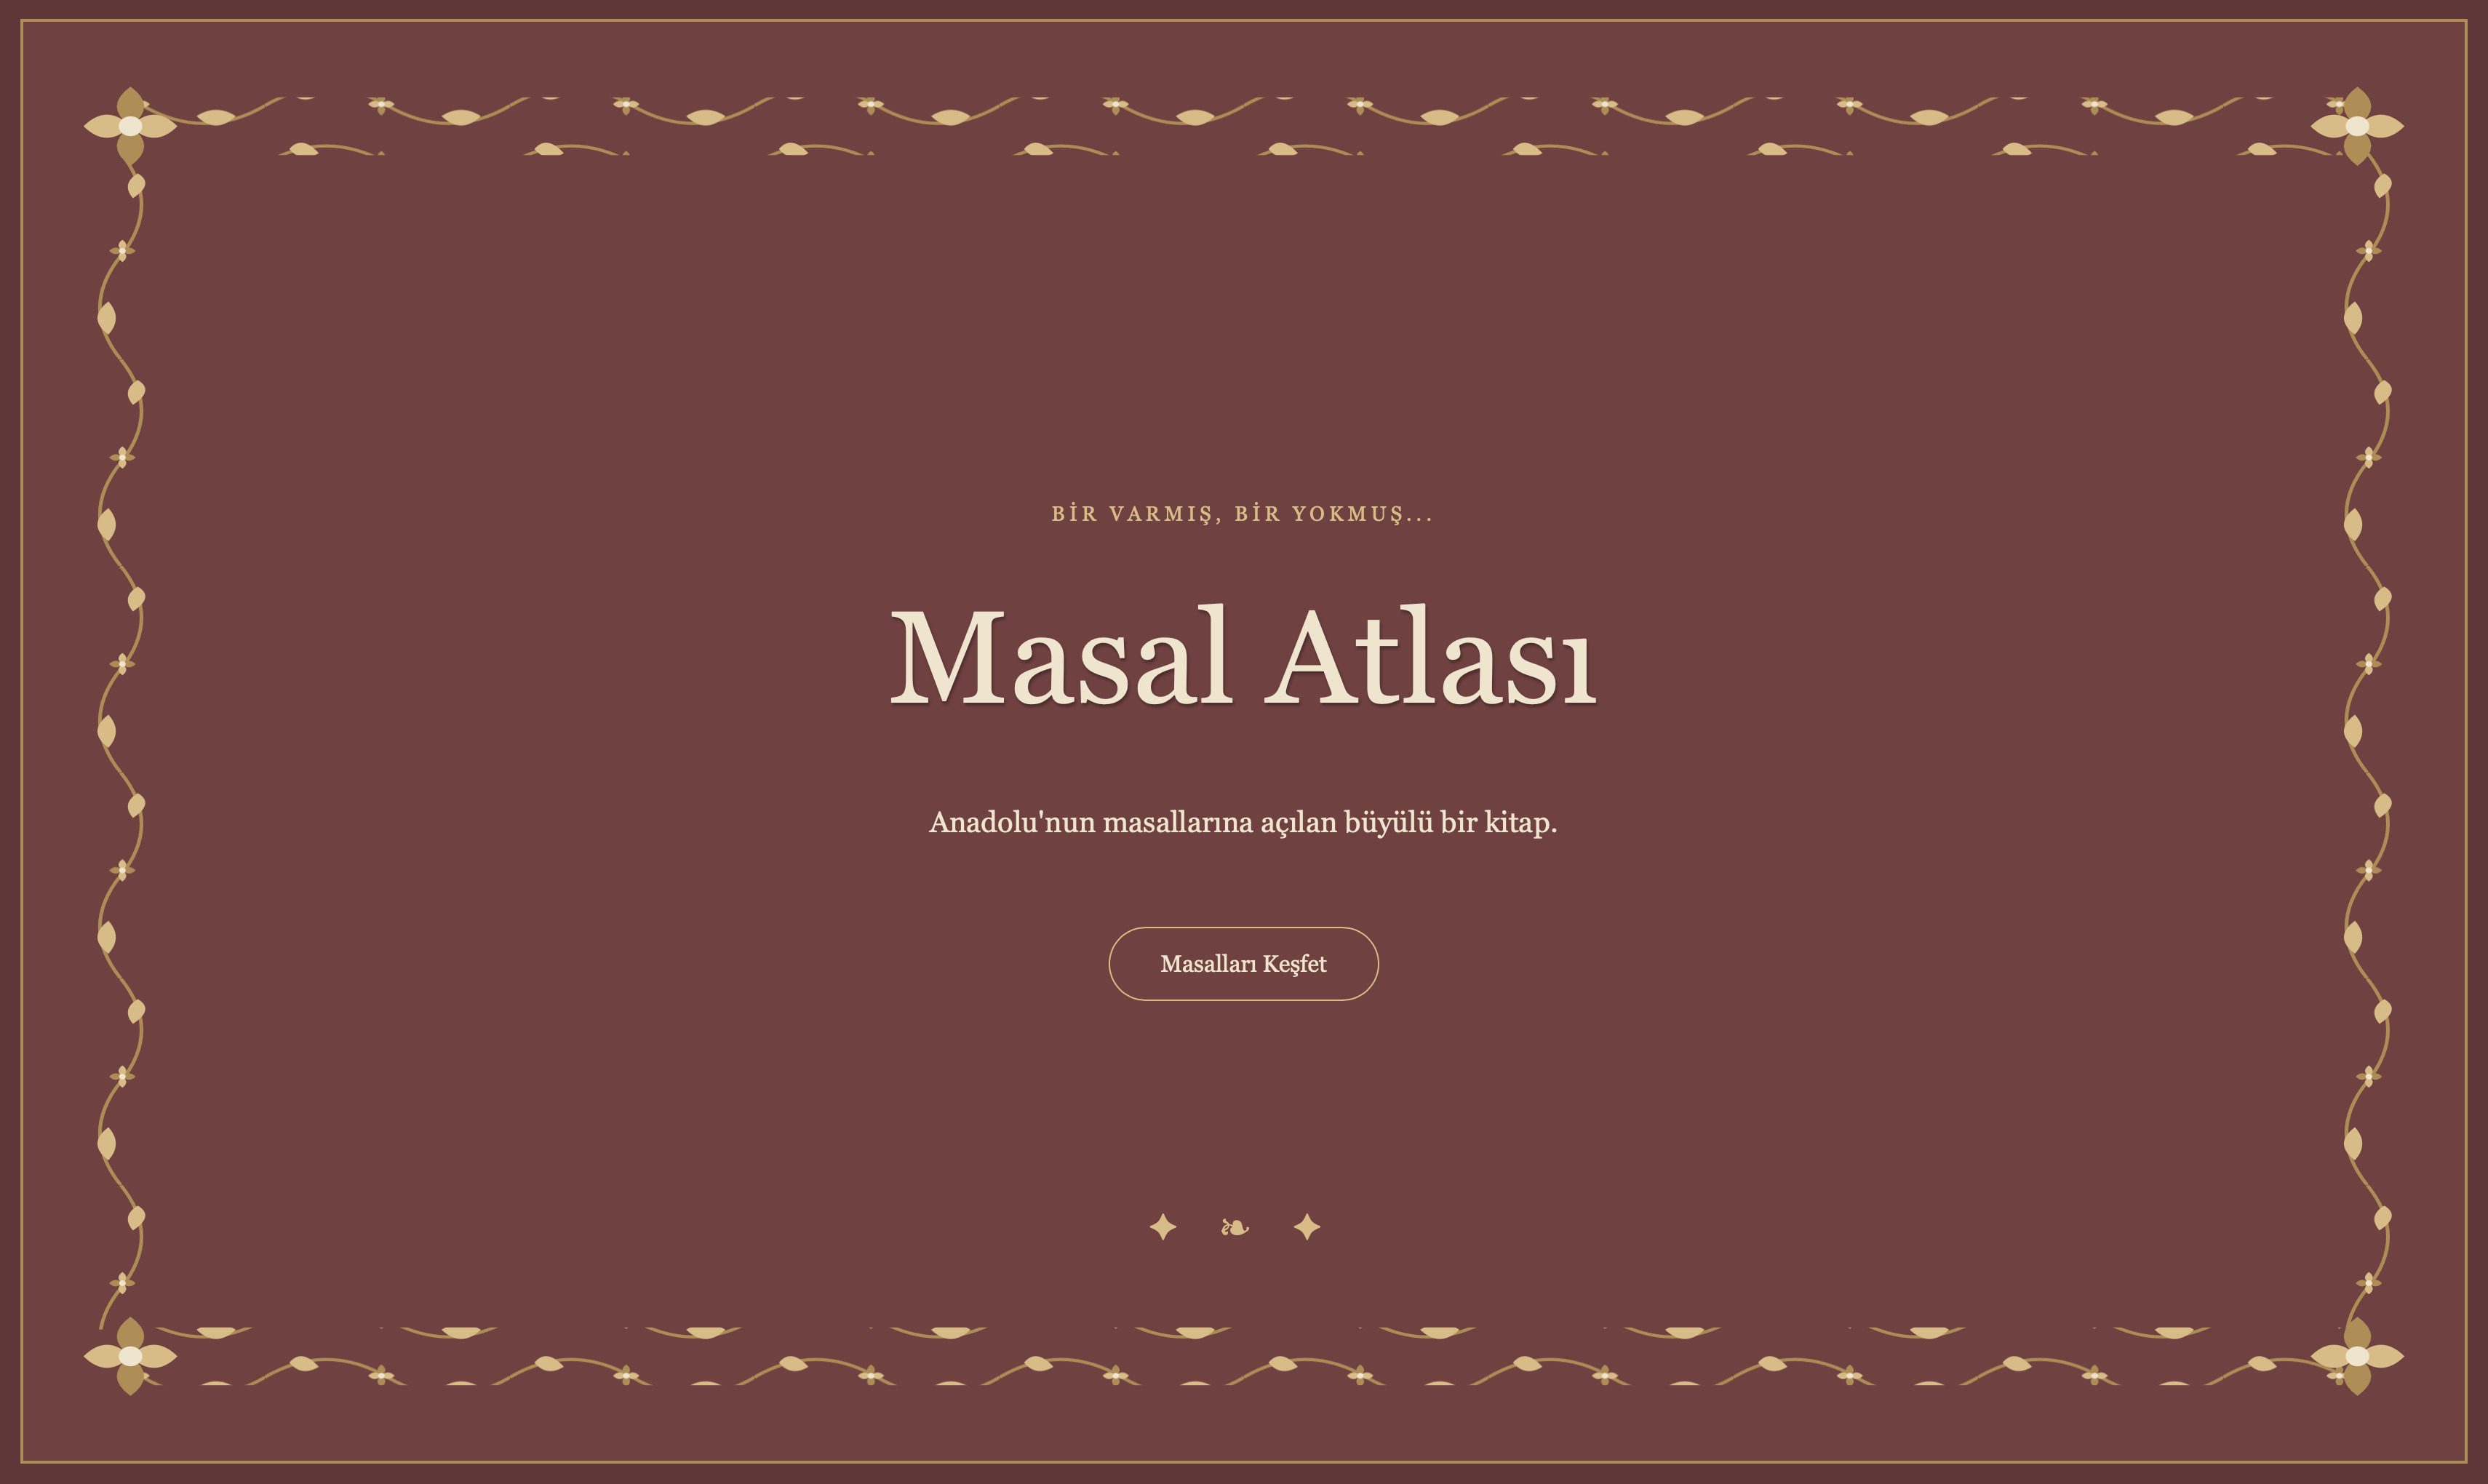
\includegraphics{ekran-ana-sayfa.png}}
\caption{Masal Atlası ana sayfa görünümü}
\end{figure}

\begin{figure}[H]
\centering
\resizebox{11cm}{!}{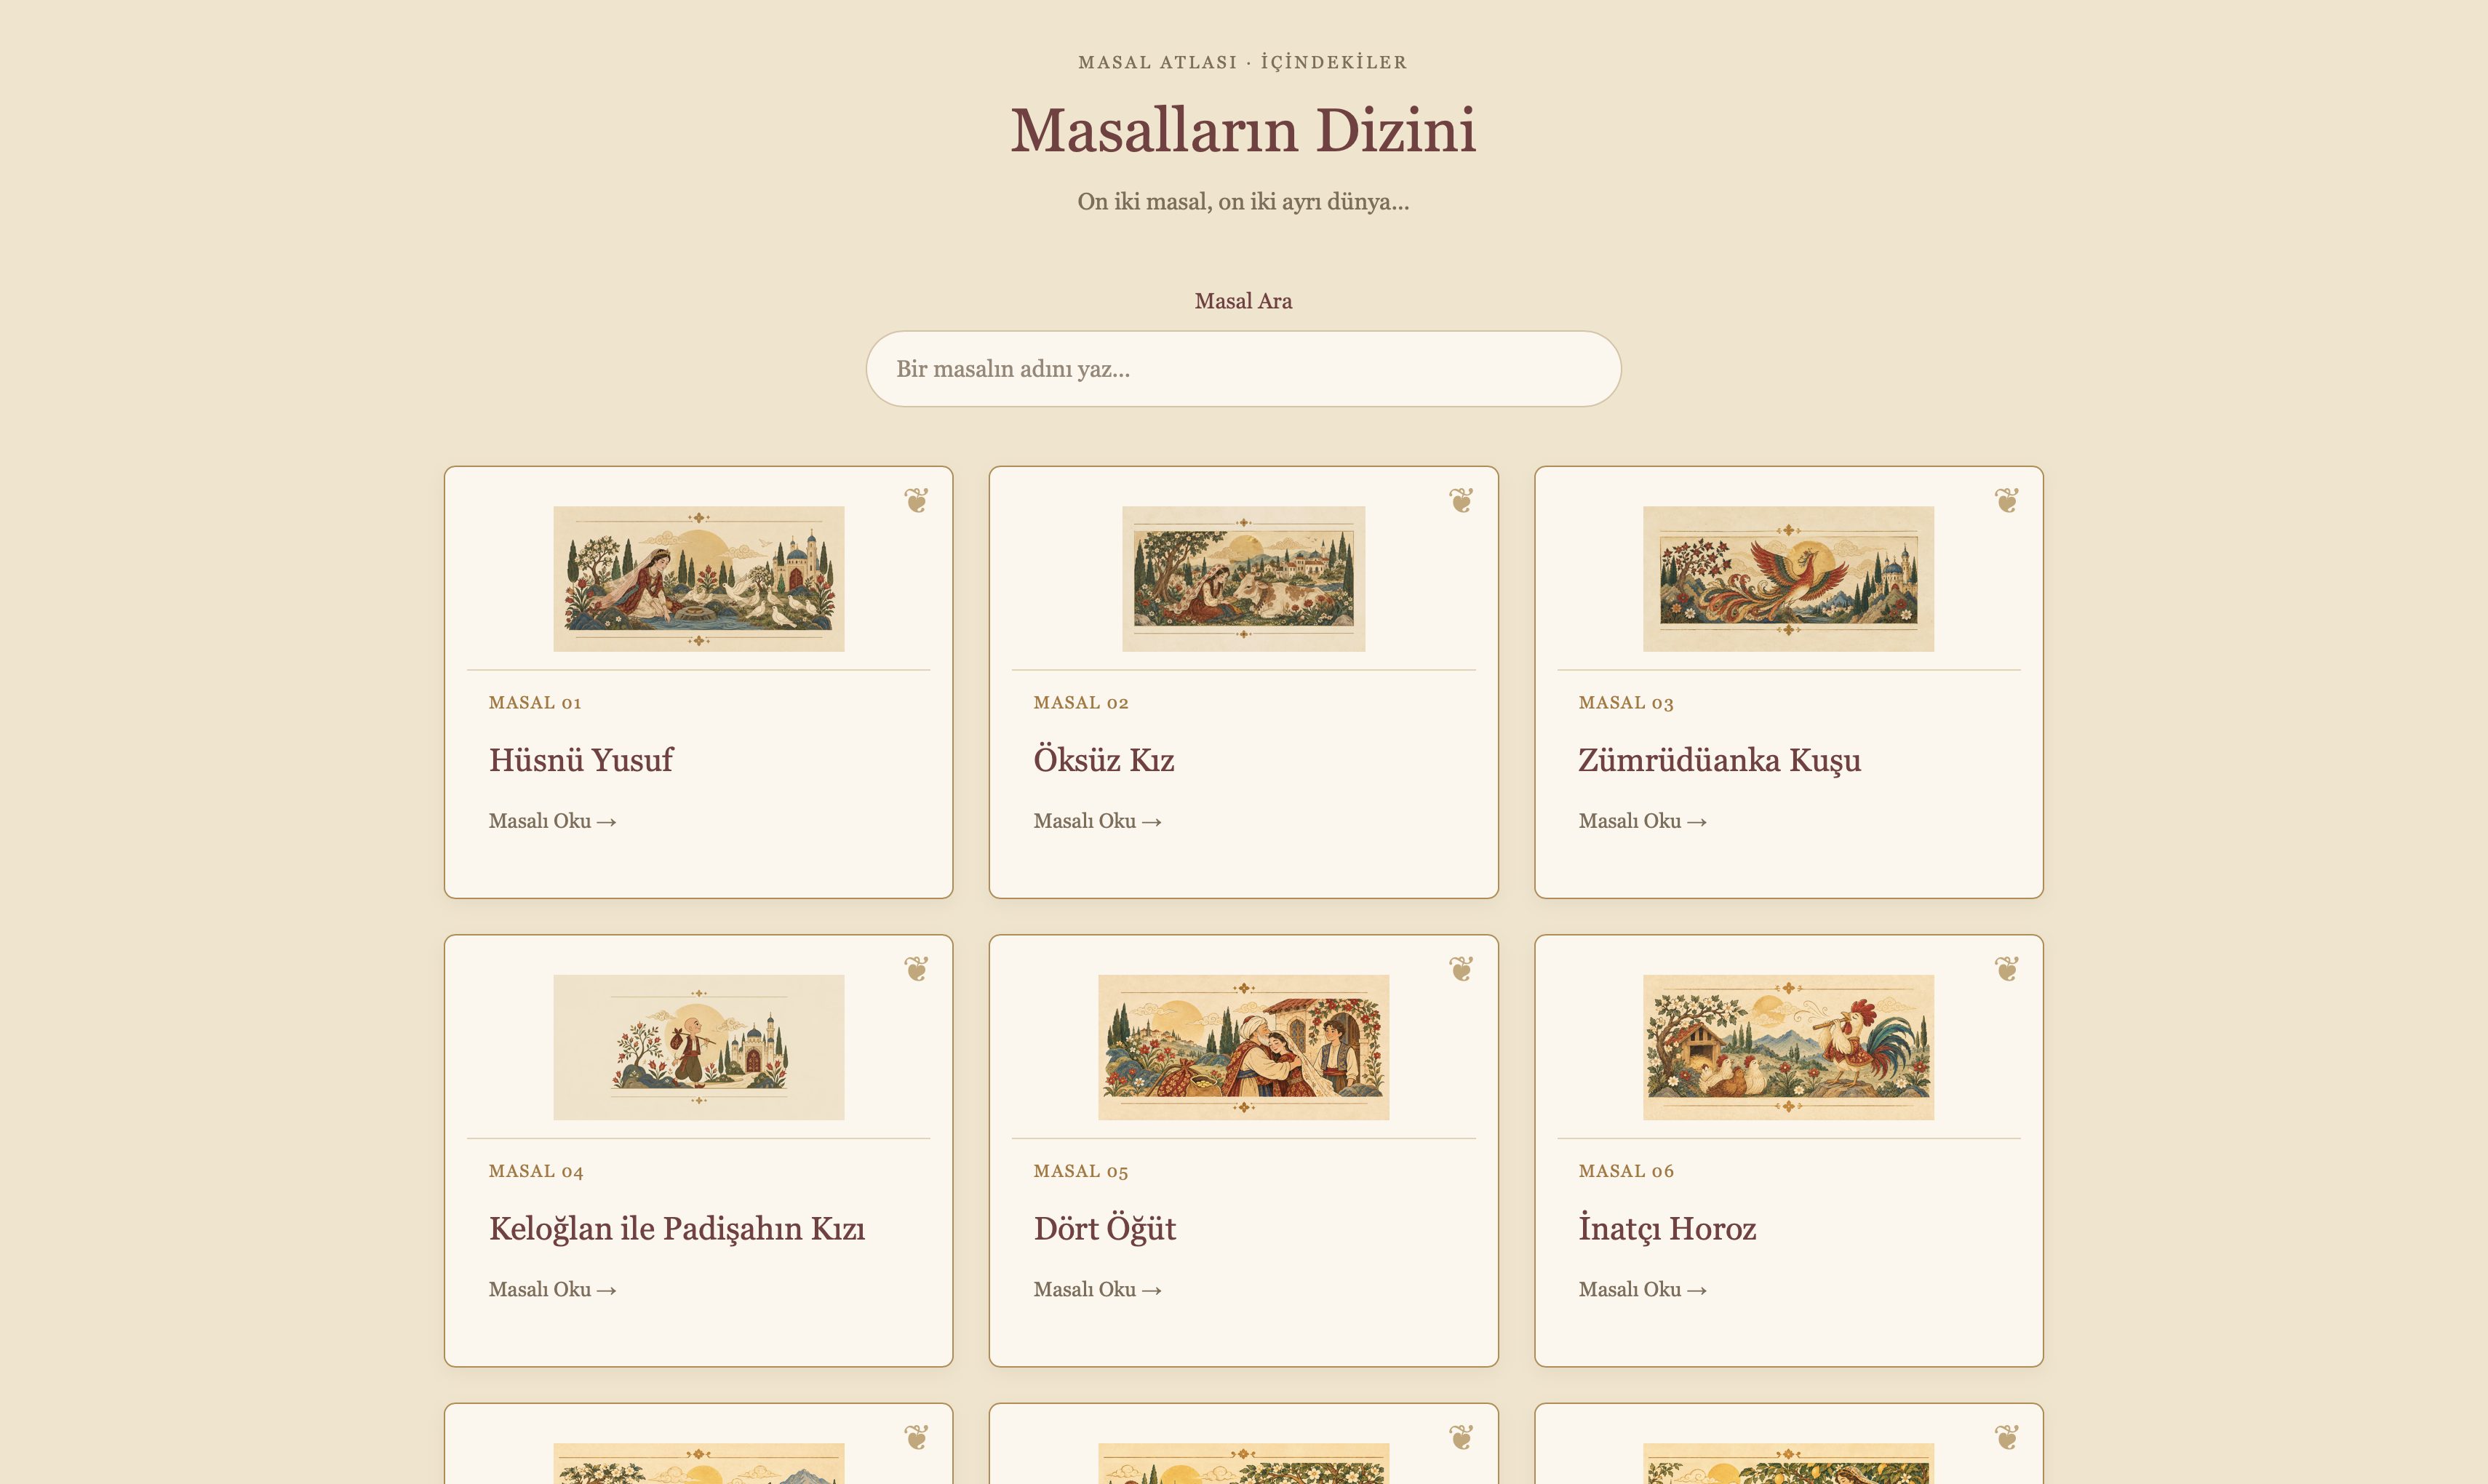
\includegraphics{ekran-masal-dizini.png}}
\caption{Masal dizini ve masal kartları}
\end{figure}

\begin{figure}[H]
\centering
\resizebox{11cm}{!}{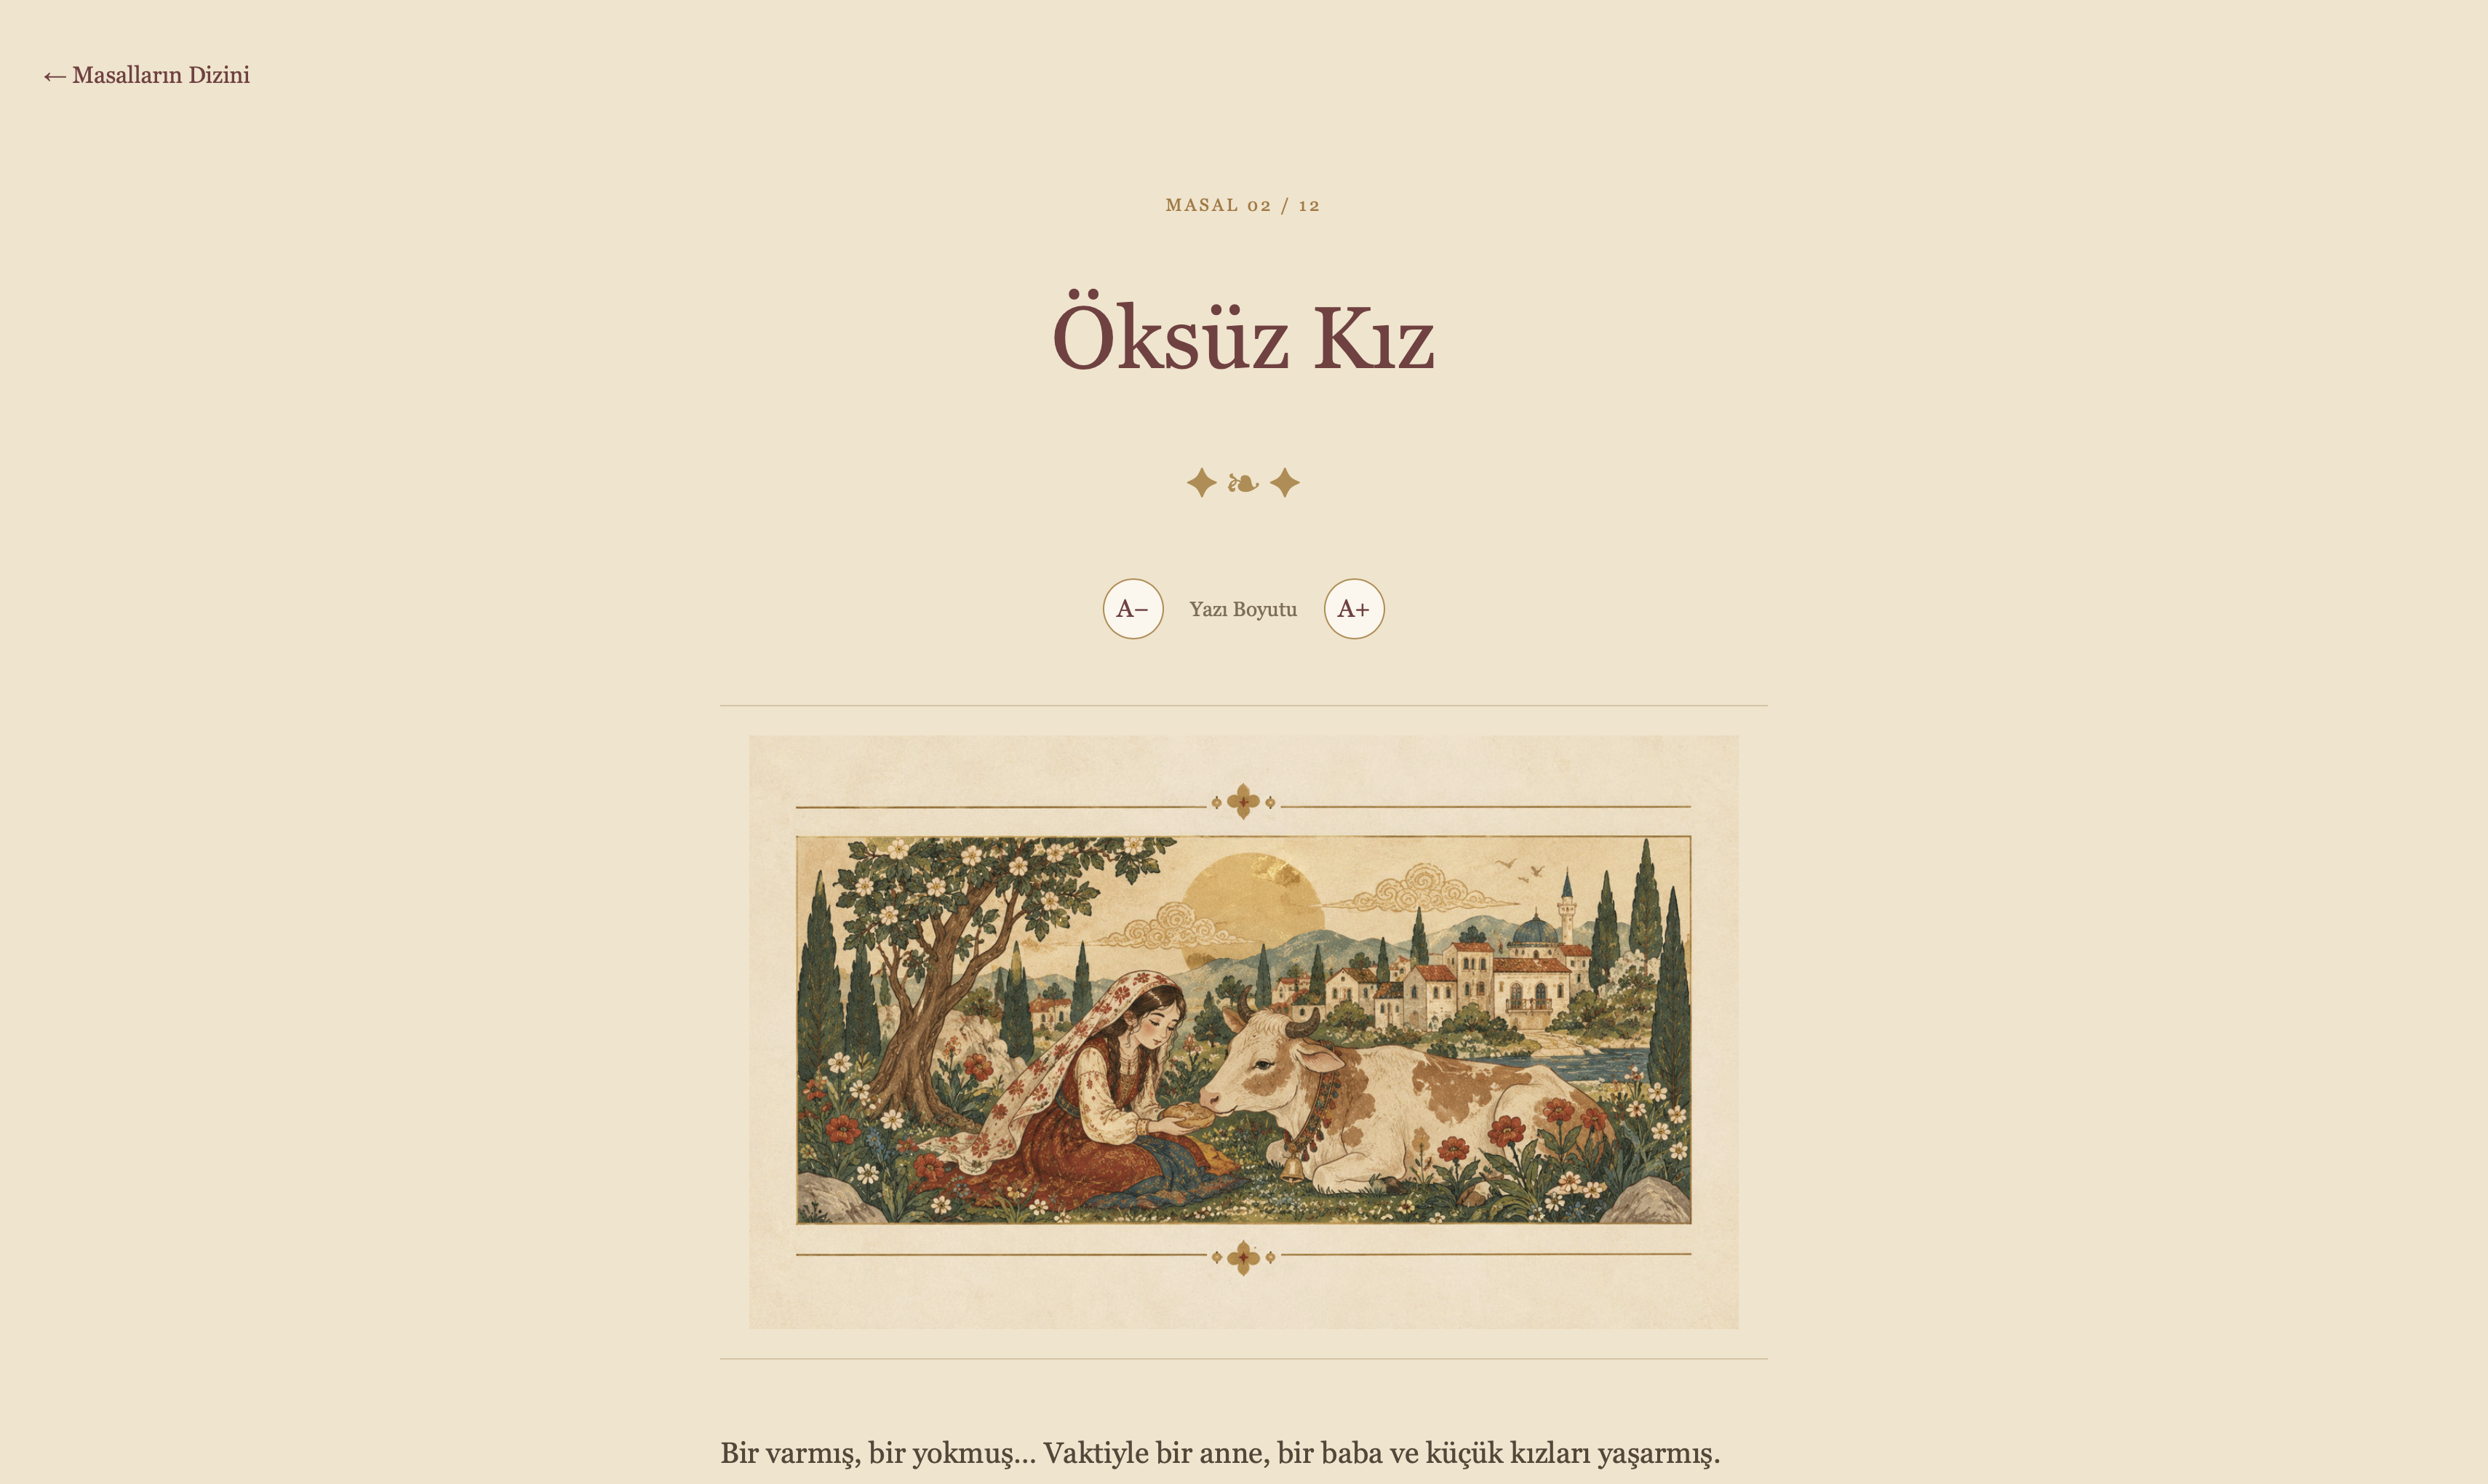
\includegraphics{ekran-masal-okuma1.png}}
\caption{Masal okuma ekranı - birinci görünüm}
\end{figure}

\begin{figure}[H]
\centering
\resizebox{11cm}{!}{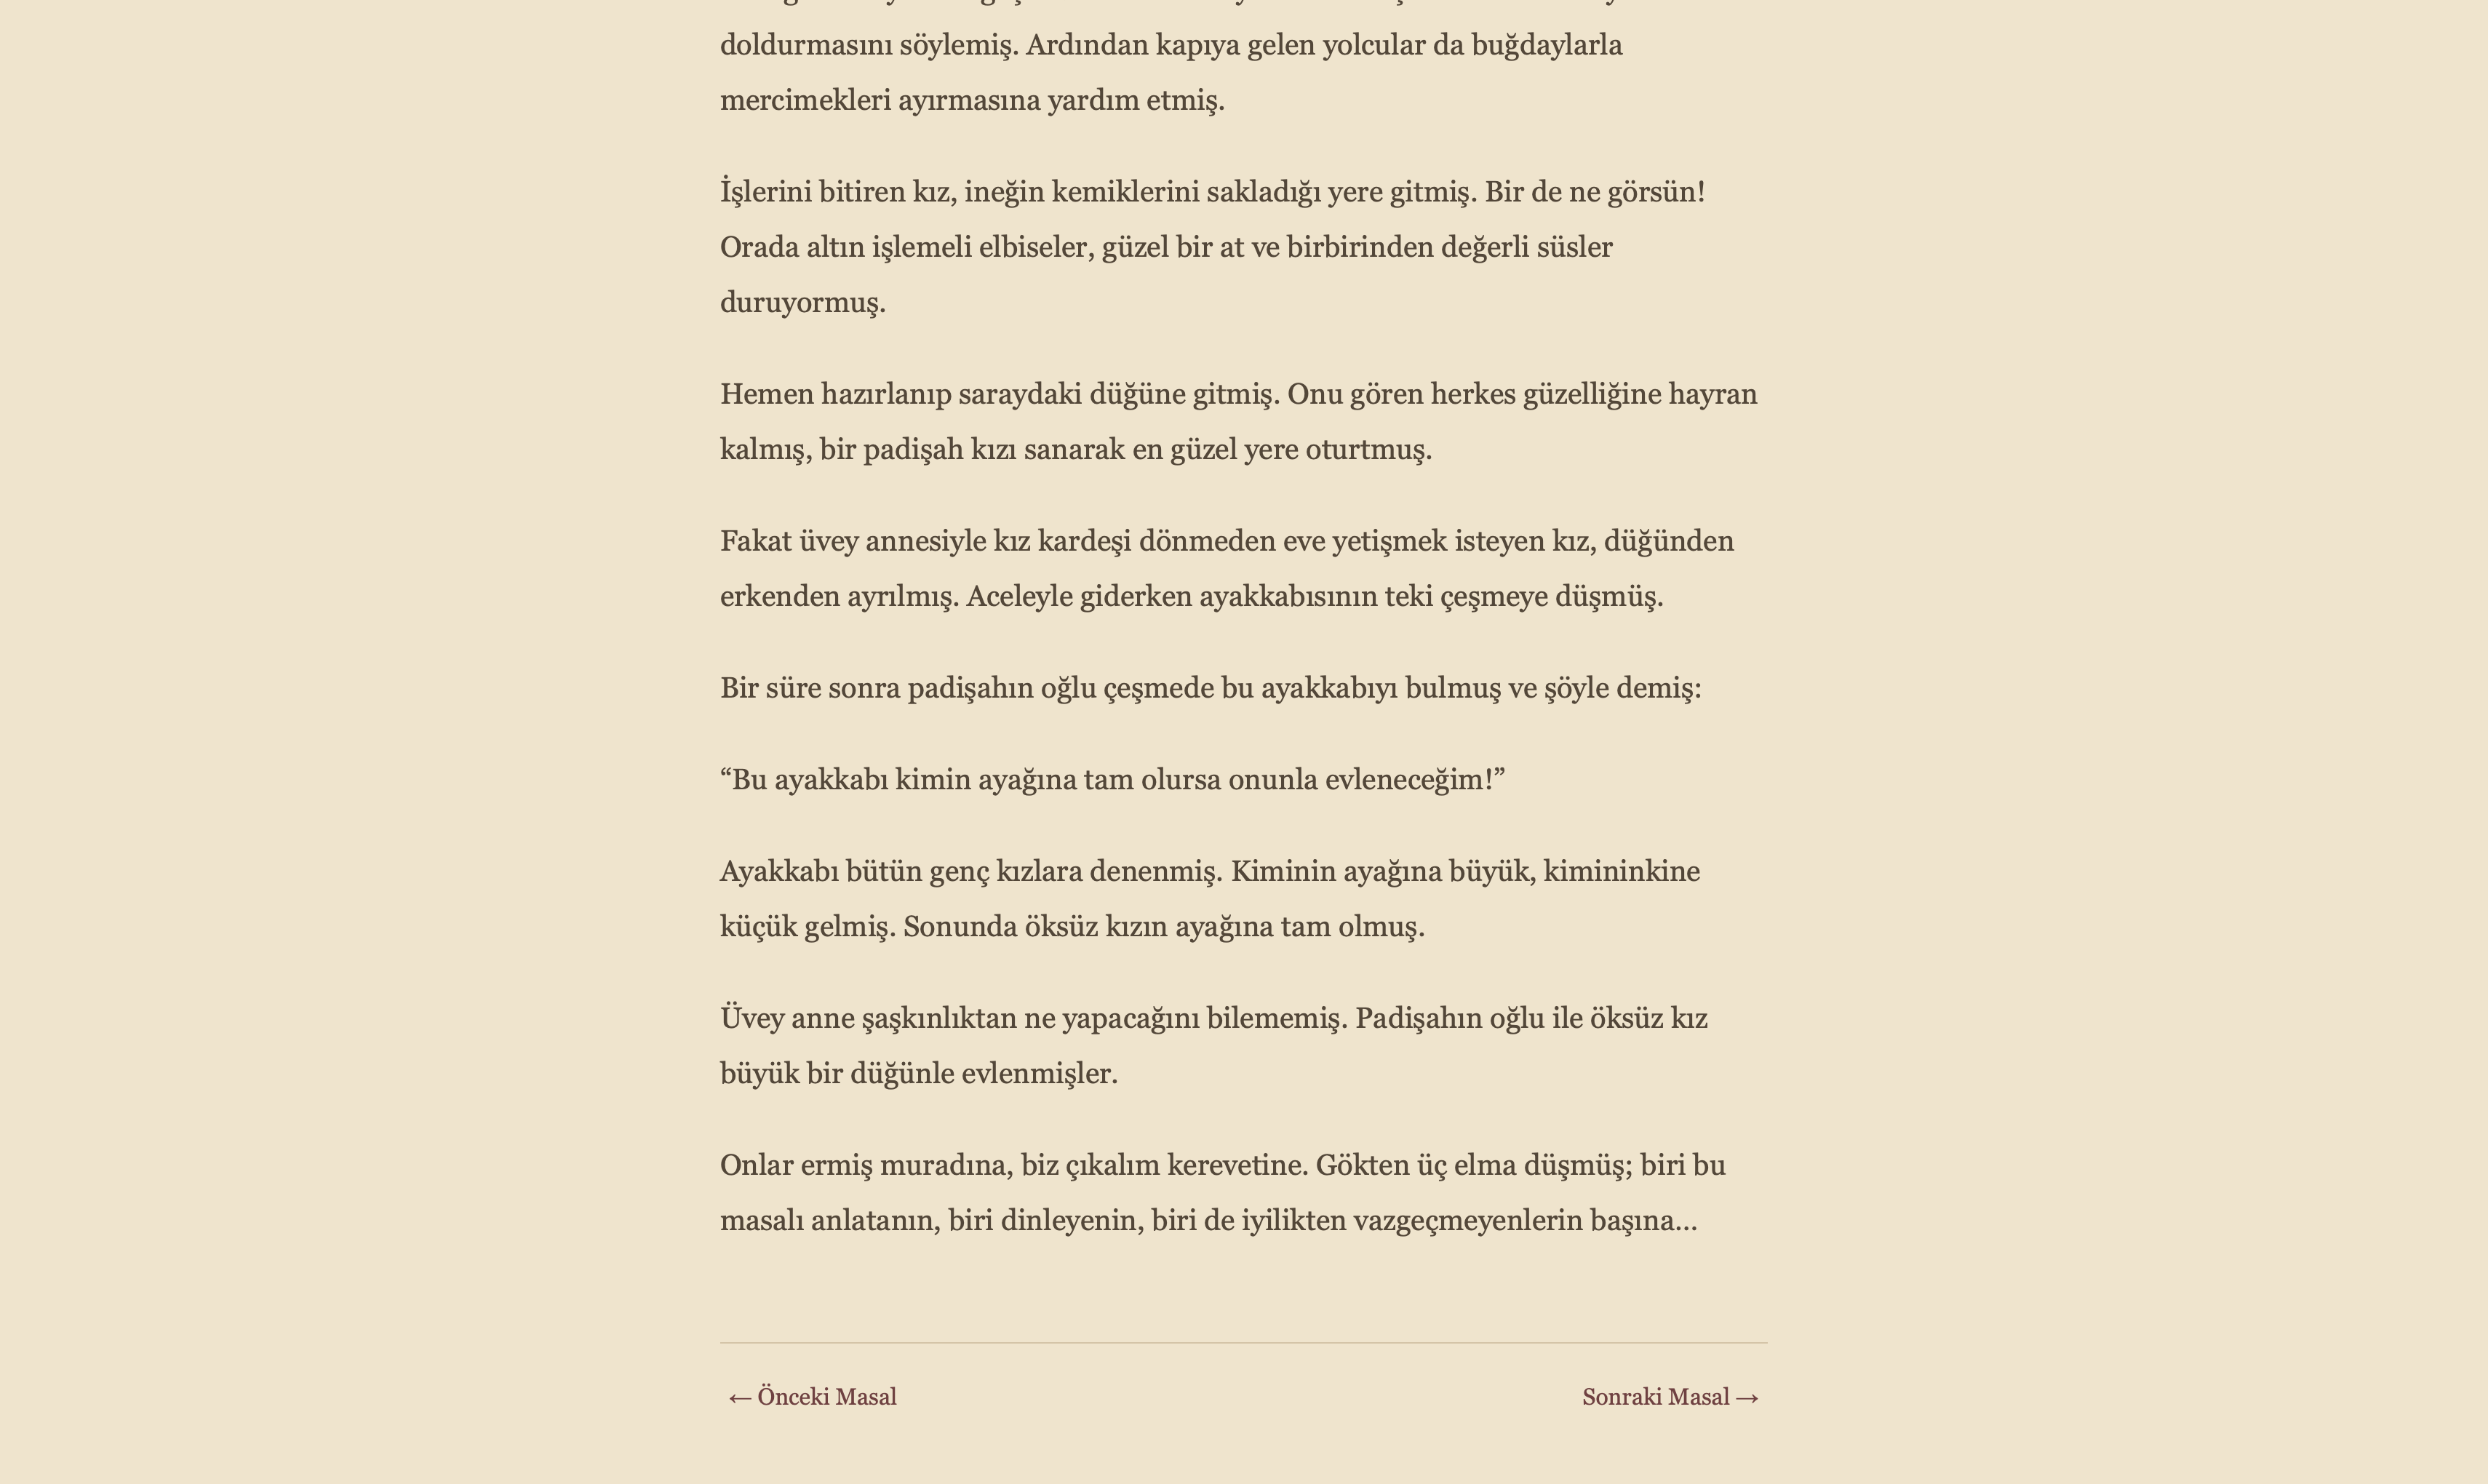
\includegraphics{ekran-masal-okuma2.png}}
\caption{Masal okuma ekranı - ikinci görünüm}
\end{figure}

\begin{figure}[H]
\centering
\resizebox{4cm}{!}{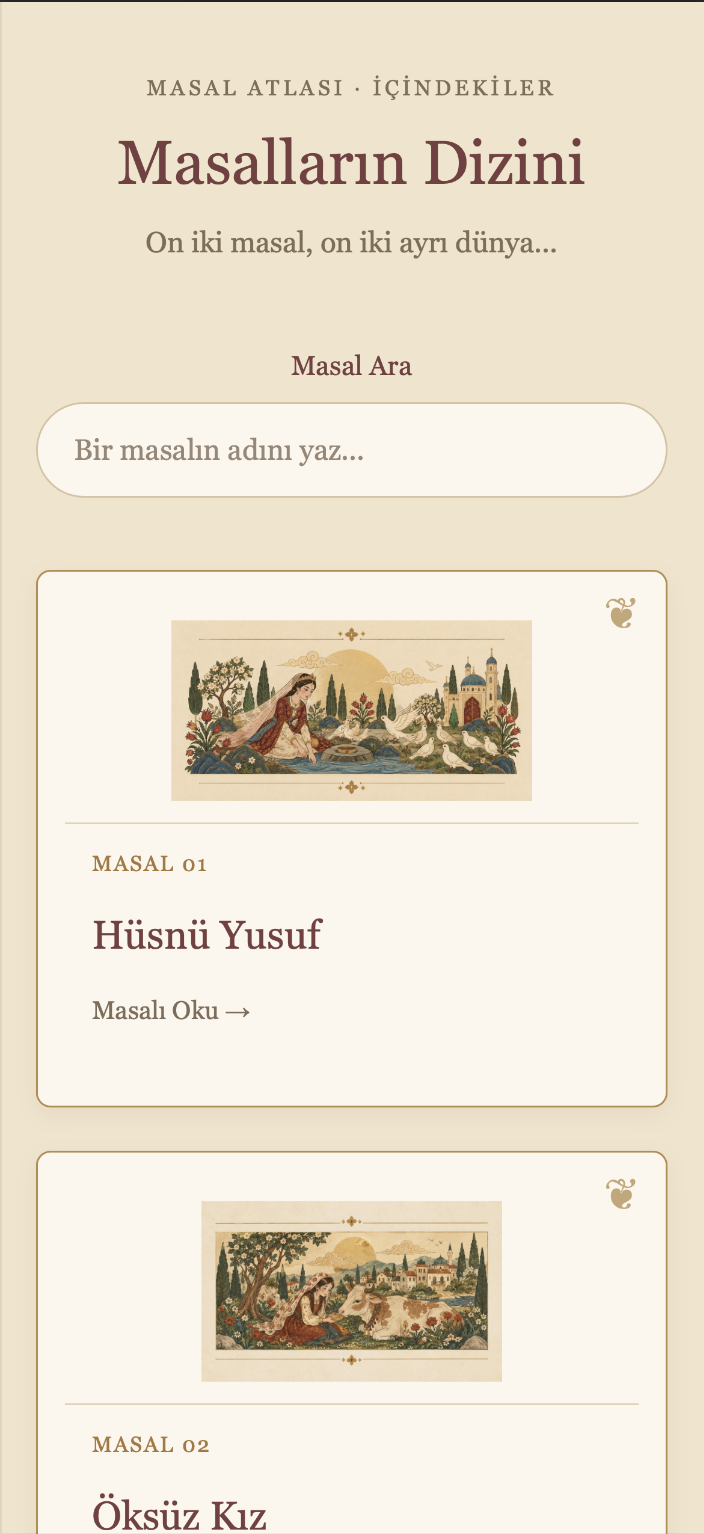
\includegraphics{ekran-mobil1.png}}
\caption{Mobil cihazda birinci görünüm}
\end{figure}

\begin{figure}[H]
\centering
\resizebox{4cm}{!}{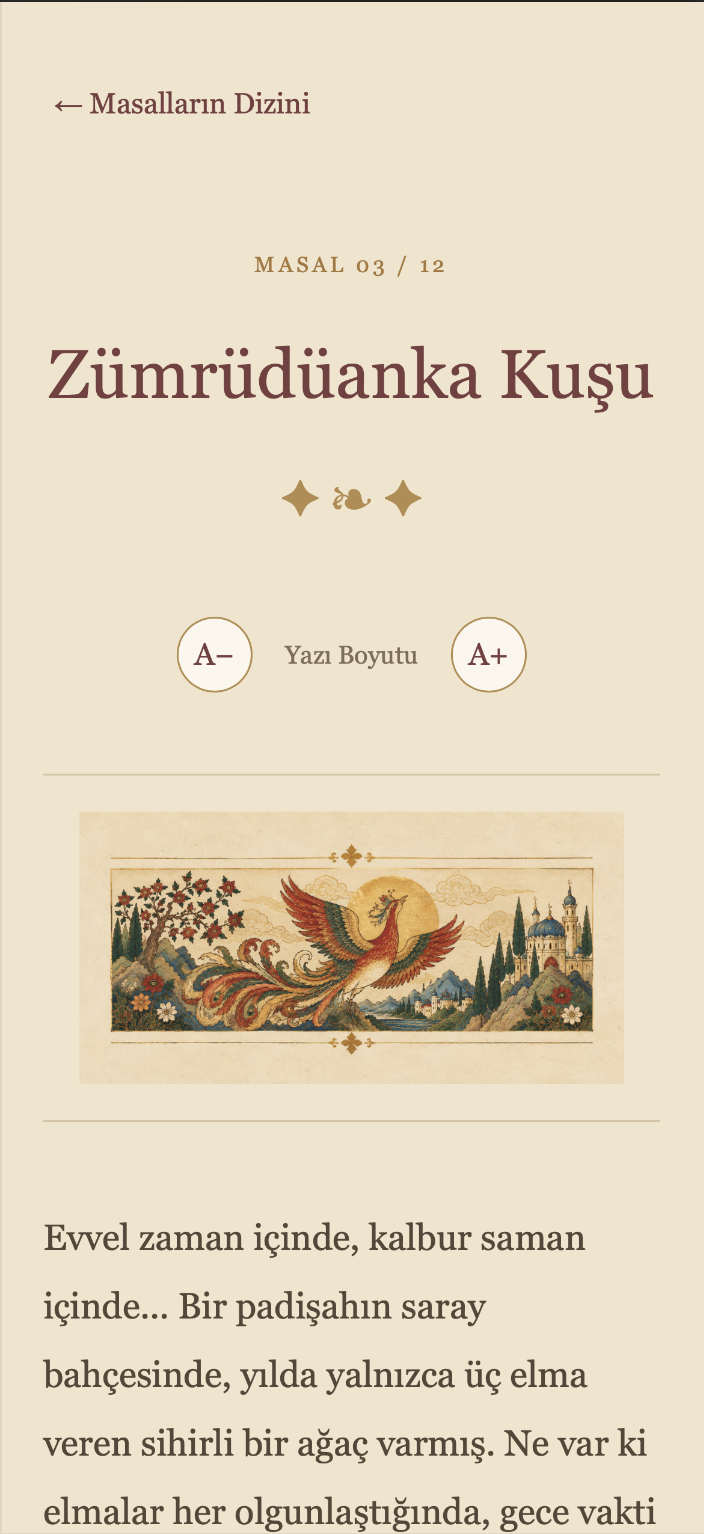
\includegraphics{ekran-mobil2.png}}
\caption{Mobil cihazda ikinci görünüm}
\end{figure}

\clearpage


% ====================================================================
\section{Gerçekleştirme}
% ====================================================================
\aciklama{Sayfanın nasıl çalıştığını kendi cümlelerinizle anlatın. Kodu sunumda
açıklayabilmelisiniz; burada da mantığını yazın. Kodun tamamını değil, önemli
bölümlerini kısa örneklerle gösterin.}

{Masal Atlası web sitesi, HTML, CSS ve JavaScript
teknolojileri kullanılarak geliştirilmiştir. Projenin
kodlama süreci Visual Studio Code üzerinde yürütülmüş;
sayfanın yapısı, görsel tasarımı ve etkileşimli
özellikleri tek bir HTML dosyası içerisinde
oluşturulmuştur.

Geliştirme sürecinde öncelikle giriş ekranı, masal
dizini ve okuma ekranının temel yapıları hazırlanmıştır.
Ardından renkler, tipografi, dekoratif çerçeveler ve
masal illüstrasyonları tasarıma eklenmiştir. JavaScript
kullanılarak masal kartlarının açılması, başlığa göre
arama yapılması, masallar arasında geçiş ve yazı
boyutunun değiştirilmesi gibi işlevler geliştirilmiştir.

Projenin farklı ekran boyutlarında düzgün
görüntülenebilmesi için duyarlı tasarım düzenlemeleri
yapılmıştır. Özellikle illüstrasyonların yerleşimi,
görsel taşmaları ve okuma ekranındaki düzen üzerinde
çeşitli testler gerçekleştirilerek karşılaşılan
sorunlar giderilmiştir. Böylece hem görsel bütünlüğü
koruyan hem de kullanıcıların rahatça masal
okuyabildiği etkileşimli bir web deneyimi
oluşturulması hedeflenmiştir.}

\subsection{HTML Yapısı}
Masal Atlası web sayfasının HTML yapısı, kullanıcıların masallara kolayca ulaşabilmesi ve rahat bir okuma deneyimi yaşayabilmesi amacıyla oluşturulmuştur. Sayfa; giriş ekranı, masalların listelendiği dizin bölümü ve seçilen masalın görüntülendiği okuma ekranı olmak üzere üç temel bölümden oluşmaktadır.

Giriş ekranında projenin başlığı, kısa bir tanıtım metni ve kullanıcıyı masalların bulunduğu bölüme yönlendiren “Masalları Keşfet” butonu yer almaktadır. Masal dizininde 12 farklı Türk masalı, başlıkları ve illüstrasyonlarıyla birlikte kartlar halinde sunulmaktadır. Kullanıcı bir masal seçtiğinde ilgili masalın başlığı, görseli ve metni okuma ekranında görüntülenmektedir.

HTML yapısında başlıklar için 'h1', 'h2' ve 'h3', açıklama ve masal metinleri için 'p', masal kartları için 'article', görseller için 'img' ve sayfanın farklı bölümlerini gruplandırmak için 'div' etiketlerinden yararlanılmıştır. Bu yapı sayesinde sayfanın içerikleri düzenli bir şekilde organize edilmiş ve CSS ile JavaScript kullanılarak geliştirilmeye uygun hale getirilmiştir.

\subsection{İçsel CSS}
Masal Atlası web sayfasının görsel tasarımı, HTML dosyası içerisinde yer alan `<style>` etiketi kullanılarak oluşturulmuştur. Böylece tasarım özellikleri ayrı bir CSS dosyasına ihtiyaç duyulmadan tek bir dosya içerisinde düzenlenmiştir.

Sayfanın renk paletinde bordo (\#763E40), krem (\#F1E4CA) ve altın (\#DDBB80) tonları tercih edilmiştir. Bordo renk özellikle giriş ekranında kullanılarak geleneksel masal atmosferini desteklerken krem tonları masal dizini ve okuma ekranlarında daha rahat bir okuma deneyimi sağlamak amacıyla kullanılmıştır. Altın tonları ise butonlarda, kenarlıklarda ve dekoratif ayrıntılarda kullanılarak tasarımın bütünlüğü korunmuştur.

Masal kartlarının düzeninde CSS ile oluşturulan yerleşim kurallarından yararlanılmıştır. Kartların arka planları, boşlukları, kenarlıkları ve görsellerinin boyutları belirlenerek düzenli bir görünüm elde edilmiştir. Butonlara eklenen `hover` özellikleri sayesinde kullanıcı fareyle butonların üzerine geldiğinde renk değişimi gerçekleşmektedir.

Ayrıca farklı ekran boyutlarında kullanılabilirliği sağlamak amacıyla duyarlı tasarım kuralları uygulanmıştır. Bilgisayar ekranında birden fazla sütun halinde görüntülenen masal kartları, telefon ekranında tek sütun halinde sıralanmaktadır. Böylece görsellerin ve metinlerin küçük ekranlarda da okunabilir olması sağlanmıştır.

\begin{lstlisting}[caption={İçsel CSS'ten önemli bir bölüm}]

.masal-dizini {
  background-color: #F1E4CA;
  padding: 90px 24px;
  min-height: 100vh;
}

.kesfet:hover {
  background-color: #B48B4D;
  color: #26394A;
}

\end{lstlisting}

\subsection{İçsel JavaScript}
Masal Atlası web sayfasının etkileşimli özellikleri, HTML dosyası içerisinde bulunan JavaScript kodlarıyla geliştirilmiştir. JavaScript sayesinde kullanıcıların masallar arasında gezinmesi, istedikleri masalı araması ve okuma ekranındaki yazı boyutunu değiştirmesi sağlanmıştır.

Web sayfasında bulunan 12 masalın metinleri JavaScript içerisinde bir dizi halinde tutulmaktadır. Kullanıcı masal kartlarından birine tıkladığında `masalAc(index)` fonksiyonu çalışarak seçilen masalın başlığını, metnini ve illüstrasyonunu okuma ekranında görüntülemektedir. Böylece her masal için ayrı bir HTML sayfası oluşturulmasına gerek kalmamıştır.

Masal dizininde bulunan arama özelliği sayesinde kullanıcılar masal başlıklarına göre arama yapabilmektedir. Ayrıca okuma ekranındaki yazı boyutunu artırma ve azaltma butonları, kullanıcıların metinleri kendi tercihlerine göre düzenlemesine olanak tanımaktadır. Sayfalar arasındaki geçişler de JavaScript ile kontrol edilerek kullanıcıların giriş ekranı, masal dizini ve okuma ekranı arasında kolayca gezinmesi sağlanmıştır.

\begin{lstlisting}[caption={İçsel JavaScript'ten önemli bir bölüm}]
function masalAc(index) {
    aktifMasal = index;

    document.getElementById("masal-basligi")
        .textContent = masallar[index];
}
\end{lstlisting}

\subsection{Sayfanın Özellikleri}

Masal Atlası, kullanıcıların geleneksel Türk masallarını dijital ortamda keşfetmesini ve okumasını sağlayan etkileşimli bir web sayfasıdır. Sayfada toplam 12 masal bulunmaktadır. Her masal, kendine ait başlığı ve illüstrasyonu ile masal dizininde kartlar halinde sunulmaktadır.

Kullanıcılar arama alanını kullanarak istedikleri masala başlığı üzerinden ulaşabilmektedir. Bir masal kartına tıklandığında ilgili masalın başlığı, görseli ve metni okuma ekranında görüntülenmektedir.

Okuma ekranında bulunan yazı boyutunu artırma ve azaltma butonları sayesinde kullanıcılar metni kendi okuma tercihlerine göre düzenleyebilmektedir. Ayrıca ana sayfa, masal dizini ve okuma ekranı arasında geçiş yapılabilmektedir.

Web sayfası duyarlı tasarım yaklaşımıyla geliştirilmiştir. Böylece masaüstü ve mobil ekranlarda içeriklerin düzenli ve okunabilir biçimde görüntülenmesi amaçlanmıştır.


% ====================================================================
\section{Yapay Zekâ Kullanımı}
% ====================================================================
\aciklama{Yapay zekâ kullanımı kod ve görsel için serbesttir; koşul, çalışmanın mantığını
anlatabilmenizdir. Kullandığınız araçları aşağıya yazın. Hiç kullanmadıysanız tek
satırda ``Yapay zekâ aracı kullanılmamıştır'' yazın ve tabloyu silin.}

\begin{longtable}{@{}p{2.6cm}p{3.6cm}p{4.2cm}p{3.4cm}@{}}
\toprule
\textbf{Araç} & \textbf{Ne için kullandınız?} & \textbf{İstem (prompt) özeti} & \textbf{Sayfada nerede?} \\
\midrule
\endhead
\relax ChatGPT  & Kod & HTML yapısı & Masal dizini \\
\relax ChatGPT  & Görsel & Masallara ait illüstrasyonların hazırlanmasında yardım alınmıştır, görsellerin geleneksel Türk minyatür sanatını çağrıştıran ortak bir görsel dile sahip olması hedeflenmiştir. & Masal dizinindeki kart görsellerinde ve masal okuma ekranlarında \\
\bottomrule
\end{longtable}

\subsection{Anladığım ve Kendim Yaptığım Kısımlar}

Masal Atlası projesini geliştirirken HTML, CSS ve JavaScript'in bir web sayfasında nasıl birlikte çalıştığını daha iyi anladım. HTML ile sayfanın temel yapısının oluşturulduğunu, CSS ile görsel düzenin sağlandığını ve JavaScript ile kullanıcı etkileşimlerinin gerçekleştirildiğini uygulamalı olarak deneyimledim.

Projenin konusunu, masal seçkisini ve genel görsel yaklaşımını kendim belirledim. Geleneksel Türk masallarını dijital ortamda sunarken Türk minyatür sanatından esinlenen bir tasarım dili kullanmayı tercih ettim. Bordo, krem ve altın tonlarından oluşan renk paletini seçerek sayfanın bütününde tutarlı bir görünüm oluşturmaya çalıştım.

Kodlama sürecinde yapay zekâdan destek alsam da oluşturulan kodları Visual Studio Code üzerinden inceleyerek sayfada hangi işlevi gerçekleştirdiklerini anlamaya çalıştım. Özellikle masal kartlarının oluşturulması, masal seçildiğinde ilgili içeriğin görüntülenmesi, arama özelliği ve yazı boyutu kontrollerinin çalışma mantığını öğrendim.

Sayfanın görsel düzenini ve kullanıcı deneyimini değerlendirerek gerekli değişiklikleri yaptım. Masaüstü ve mobil görünümleri tarayıcı üzerinden test ettim. Karşılaştığım sorunlarda farklı çözümleri deneyerek sayfanın daha düzenli ve kullanılabilir hale gelmesini sağladım.

Bu süreçte yapay zekâdan yalnızca hazır sonuç almak için değil, kodlama mantığını öğrenmek ve karşılaştığım sorunları çözmek için de yararlandım. Projenin tasarım kararlarını, içerik düzenini ve son kontrollerini kendim gerçekleştirerek ortaya çıkan çalışmayı geliştirdim.


% ====================================================================
\section{Haftalık Katkılar}
% ====================================================================
\aciklama{Her hafta ders içinde yaptığınız çalışmayı kısaca yazın (2--4 cümle). Hangi
özelliği eklediğinizi ya da neyi düzelttiğinizi belirtin ve ilgili commit mesajını
ya da bağlantısını ``Commit'' satırına yazın. Her satıra ekran görüntüsü ekleyin:
resimleri \texttt{hafta1.png}, \texttt{hafta2.png}, \ldots{} adıyla Overleaf
projesine yükleyin. Aynı haftaya ikinci bir görsel eklemek için
\texttt{hafta1b.png} gibi bir dosya yükleyin; kendiliğinden görünür.
Her haftanın altındaki kutulardan o hafta için geçerli olanı $\boxtimes$ ile
işaretleyin: dersin kendisinde katılım gösterdiyseniz ``Ders içinde katılım
sergiledim'', o haftayı sonradan tamamladıysanız ``Telafi yaptım''. Telafi
yaptıysanız yapılan çalışmanın metninde bunu açıkça belirtin.}


\begin{longtable}{@{}>{\raggedright\arraybackslash}m{1.7cm}
                    >{\raggedright\arraybackslash}m{6.4cm}
                    >{\centering\arraybackslash}m{6cm}@{}}

\toprule
\rowcolor{ana}\textcolor{white}{\textbf{Hafta}} & \textcolor{white}{\textbf{Yapılan çalışma}} & \textcolor{white}{\textbf{Görsel}} \\
\midrule
\endfirsthead
\toprule
\rowcolor{ana}\textcolor{white}{\textbf{Hafta}} & \textcolor{white}{\textbf{Yapılan çalışma}} & \textcolor{white}{\textbf{Görsel}} \\
\midrule
\endhead
\bottomrule
\endfoot

\textbf{1. hafta}\newline [tarih] &
WorldWideWeb sayfasının HTML yapısını oluşturdum. Başlık, paragraf, liste ve bağlantı etiketlerini kullanarak sayfa içi gezinme özelliğini hazırladım.
\newline \textbf{Commit:} \href{https://teams.microsoft.com/l/message/19:e74f27e293aa4b83bc2233b4170b1bbe@thread.tacv2/1790854592776?tenantId=afb14aed-4a54-433f-9753-519aa64a3e48&groupId=7a5bb549-3faf-4a84-bb15-8be3b76924ba&parentMessageId=1790797426260&teamName=*26-27.86.GIT3168820.PROGRAMLAMAYA%20G%C4%B0R%C4%B0%C5%9E%20(A)&channelName=Hafta%201-2%20Kat%C4%B1l%C4%B1m%20Telafisi&createdTime=1790854592776}{Teams mesajı}
\newline $\square$ Ders içinde katılım sergiledim
\newline $\boxtimes$ Telafi yaptım &
\haftagorsel{hafta1.png} \\
\midrule
\textbf{2. hafta}\newline [tarih] &
WorldWideWeb sayfasının tasarımını içsel CSS kullanarak geliştirdim. Arka plan rengini, yazı tiplerini, bağlantı renklerini ve sayfanın genel yerleşimini düzenledim.
\newline \textbf{Commit:} \href{https://teams.microsoft.com/l/message/19:e74f27e293aa4b83bc2233b4170b1bbe@thread.tacv2/1790854592776?tenantId=afb14aed-4a54-433f-9753-519aa64a3e48&groupId=7a5bb549-3faf-4a84-bb15-8be3b76924ba&parentMessageId=1790797426260&teamName=*26-27.86.GIT3168820.PROGRAMLAMAYA%20G%C4%B0R%C4%B0%C5%9E%20(A)&channelName=Hafta%201-2%20Kat%C4%B1l%C4%B1m%20Telafisi&createdTime=1790854592776}{Teams mesajı}
\newline $\square$ Ders içinde katılım sergiledim
\newline $\boxtimes$ Telafi yaptım &
\haftagorsel{hafta2.png} \\
\midrule
\textbf{3. hafta}\newline [tarih] &
HTML ve içsel CSS kullanarak "Moda Tasarımının Dönüşümü" konulu bir web sayfası hazırladım. Sayfaya görsel, bağlantılar, listeler ve buton ekleyerek tasarımını düzenledim. Ayrıca JavaScript ile uyarı penceresi oluşturma ve buton aracılığıyla yeni sekme açma çalışmalarını gerçekleştirdim.
\newline \textbf{Commit:} \href{https://teams.microsoft.com/l/message/19:76e81a64fe6448979da4ee91dd5a3fb4@thread.tacv2/1790794142747?tenantId=afb14aed-4a54-433f-9753-519aa64a3e48&groupId=7a5bb549-3faf-4a84-bb15-8be3b76924ba&parentMessageId=1790769289077&teamName=*26-27.86.GIT3168820.PROGRAMLAMAYA%20G%C4%B0R%C4%B0%C5%9E%20(A)&channelName=Kat%C4%B1l%C4%B1m%20Telafi%20Genel&createdTime=1790794142747}{Teams mesajı}
\newline $\square$ Ders içinde katılım sergiledim
\newline $\boxtimes$ Telafi yaptım &


\haftagorsel{hafta3.png} \\

\midrule
\textbf{4. hafta}\newline [tarih] &
JavaScript kullanarak web sayfalarına etkileşim kazandırmaya yönelik çalışmalar gerçekleştirdim. Kullanıcıdan isim alarak ekranda karşılama mesajı gösteren bir giriş alanı oluşturdum ve CSS ile görsel düzenlemeler yaptım. Ayrıca butonlara tıklandığında farklı mesajlar gösteren örnekler hazırladım. Son olarak artırma, azaltma ve sıfırlama butonlarıyla çalışan basit bir sayaç uygulaması geliştirdim. Bu çalışmalar sayesinde JavaScript olaylarını ve HTML içeriğini dinamik olarak değiştirmeyi öğrendim.
\newline \textbf{Commit:} \href{https://teams.microsoft.com/l/message/19:76e81a64fe6448979da4ee91dd5a3fb4@thread.tacv2/1791392060067?tenantId=afb14aed-4a54-433f-9753-519aa64a3e48&groupId=7a5bb549-3faf-4a84-bb15-8be3b76924ba&parentMessageId=1791361594974&teamName=*26-27.86.GIT3168820.PROGRAMLAMAYA%20G%C4%B0R%C4%B0%C5%9E%20(A)&channelName=Kat%C4%B1l%C4%B1m%20Telafi%20Genel&createdTime=1791392060067}{Teams mesajı}
\newline $\square$ Ders içinde katılım sergiledim
\newline $\boxtimes$ Telafi yaptım &
\haftagorsel{hafta4a.png}\haftaek{hafta4b.png} \\
\midrule
\textbf{5. hafta}\newline [tarih] &
HTML, CSS ve JavaScript kullanarak etkileşimli bir kutu uygulaması hazırladım. Sayfaya dört farklı kutu yerleştirdim ve CSS ile renklerini, boyutlarını ve görünümlerini düzenledim. JavaScript ile butonlara tıklanmasını algılayan olay dinleyicileri oluşturarak kutuların renk değiştirmesini sağladım. Bu çalışma sayesinde kullanıcı etkileşimlerine bağlı olarak sayfa elemanlarının görsel özelliklerini değiştirmeyi öğrendim.
\newline \textbf{Commit:} \href{https://teams.microsoft.com/l/message/19:76e81a64fe6448979da4ee91dd5a3fb4@thread.tacv2/1791993066006?tenantId=afb14aed-4a54-433f-9753-519aa64a3e48&groupId=7a5bb549-3faf-4a84-bb15-8be3b76924ba&parentMessageId=1791960451608&teamName=*26-27.86.GIT3168820.PROGRAMLAMAYA%20G%C4%B0R%C4%B0%C5%9E%20(A)&channelName=Kat%C4%B1l%C4%B1m%20Telafi%20Genel&createdTime=1791993066006}{Teams mesajı}
\newline $\square$ Ders içinde katılım sergiledim
\newline $\boxtimes$ Telafi yaptım &
\haftagorsel{hafta5.png}\haftaek{hafta5b.png} \\
\midrule
\textbf{6. hafta}\newline [tarih] &
Bu hafta HTML ve harici CSS kullanarak "Atölye Notları" isimli bir web sayfası hazırladım. CSS kodlarını HTML dosyasından ayrı bir dosyada düzenleyerek bağlantı kurmayı öğrendim. Sayfada başlık, hakkında ve alt bilgi bölümleri oluşturdum. Arka plan renklerini, yazı tiplerini, boşlukları ve bölümlerin görsel düzenini CSS ile şekillendirdim. Bu çalışma sayesinde harici CSS kullanımının kodların daha düzenli ve yönetilebilir olmasını sağladığını öğrendim.
\newline \textbf{Commit:} \href{https://teams.microsoft.com/l/message/19:76e81a64fe6448979da4ee91dd5a3fb4@thread.tacv2/1792587369162?tenantId=afb14aed-4a54-433f-9753-519aa64a3e48&groupId=7a5bb549-3faf-4a84-bb15-8be3b76924ba&parentMessageId=1792565991141&teamName=*26-27.86.GIT3168820.PROGRAMLAMAYA%20G%C4%B0R%C4%B0%C5%9E%20(A)&channelName=Kat%C4%B1l%C4%B1m%20Telafi%20Genel&createdTime=1792587369162}{Teams mesajı}
\newline $\square$ Ders içinde katılım sergiledim
\newline $\boxtimes$ Telafi yaptım &
\haftagorsel{hafta6.png}\haftaek{hafta6b.png} \\
\midrule
\textbf{7. hafta}\newline [tarih] &
[Bu hafta yaptığınız çalışma.]\newline \textbf{Commit:} [mesaj veya bağlantı]\katilimkutulari &
\haftagorsel{hafta7.png}\haftaek{hafta7b.png} \\
\midrule
\textbf{8. hafta}\newline [tarih] &
[Bu hafta yaptığınız çalışma.]\newline \textbf{Commit:} [mesaj veya bağlantı]\katilimkutulari &
\haftagorsel{hafta8.png}\haftaek{hafta8b.png} \\
\end{longtable}

% ====================================================================
\section{Test ve Değerlendirme}
% ====================================================================
Masal Atlası web sayfasını Google Chrome ve Safari
tarayıcılarında test ettim. Bilgisayar ve mobil ekran
boyutlarında sayfanın görünümünü inceledim. Ana sayfa,
masal dizini, masal okuma ekranı, arama özelliği ve
yazı boyutu değiştirme butonlarını kontrol ettim.
Ayrıca farklı ekran genişliklerinde tasarımın
uyumunu değerlendirdim.

\begin{center}
\rowcolors{2}{acik}{white}
\begin{tabular}{@{}p{6cm}p{3.4cm}p{3.4cm}@{}}
\toprule
\rowcolor{ana}\textcolor{white}{\textbf{Özellik}} & \textcolor{white}{\textbf{Bilgisayar}} & \textcolor{white}{\textbf{Telefon}} \\
\midrule
\relax Masal kartları ve okuma ekranı & Çalışıyor & Çalışıyor \\
\relax Masal arama özelliği & Çalışıyor & Çalışıyor \\
\relax Yazı boyutu değiştirme & Çalışıyor & Çalışıyor \\
\bottomrule
\end{tabular}
\end{center}

\textbf{Denenen tarayıcılar:} Google Chrome ve Safari.

% ====================================================================
\section{Sunum Videosu}
% ====================================================================

\begin{center}
\begin{tabular}{@{}ll@{}}
\textbf{Video süresi:} & 14:10 (14 dakika 10 saniye) \\
\textbf{Görünürlük:} & Liste dışı \\
\textbf{Bağlantı:} & \url{https://youtu.be/0LZKcCXk2jo} \\
\end{tabular}
\end{center}

\subsection{Video Kontrol Listesi}
\aciklama{Teslimden önce hepsini kontrol edin ve kutuları $\boxtimes$ ile işaretleyin.}
\begin{itemize}
  \item $\boxtimes$ Süre 12--18 dakika aralığında.
  \item$\boxtimes$ Sunum boyunca kameram açık, yüzüm görünüyor.
  \item $\boxtimes$ Görünürlük \textbf{Listelenmemiş} (ya da Herkese açık); \textbf{Özel} değil.
  \item $\boxtimes$ Bağlantıyı gizli pencerede açtım, video oynuyor.
  \item $\boxtimes$ YouTube videoyu işlemeyi bitirdi.
  \item $\boxtimes$ Videoyu baştan sona izledim; ses ve kamera tüm sunumda var.
  \item $\boxtimes$ Kapaktaki bağlantı ile bu bölümdeki bağlantı aynı.
\end{itemize}

% ====================================================================
\section{Sonuç ve Kendi Değerlendirmem}
% ====================================================================
\aciklama{Projeden ne öğrendiniz? En çok nerede zorlandınız ve nasıl çözdünüz? İleride
neyi geliştirirdiniz? 6--10 cümle yeterlidir.}

Masal Atlası projesi sayesinde HTML, CSS ve JavaScript kullanarak bir web sayfasını baştan sona oluşturma sürecini deneyimledim. Özellikle tasarım kararlarını kod aracılığıyla uygulamayı, sayfa düzenini oluşturmayı ve kullanıcı etkileşimlerini geliştirmeyi öğrendim. Proje boyunca en çok masal metinlerinin, görsellerin ve sayfalar arası geçişlerin birlikte sorunsuz çalışmasını sağlamakta zorlandım. Bu sorunları kodları tekrar inceleyerek, gerekli düzenlemeleri yaparak ve sayfayı farklı ekran boyutlarında test ederek çözmeye çalıştım. Görsel iletişim tasarımı alanında edindiğim bilgileri programlamayla birleştirmek benim için önemli bir deneyim oldu. İleride projeyi sesli masal anlatımları, farklı okuma seçenekleri ve daha fazla masal ekleyerek geliştirmek isterim.

% ====================================================================
\section{Kaynakça}
% ====================================================================
\aciklama{Masal metinleri için yararlandığınız kitap ve sitelerle, teknik kaynakları
(MDN vb.) ve kullandığınız görsel kaynaklarını yazın. Masalları kendi
cümlelerinizle yazmanız gerekir; kaynaklar yalnızca yararlandığınız yerleri
gösterir.}

\begin{thebibliography}{9}
\bibitem{k1} https://www.kulturportali.gov.tr/portal/masallar-1
\bibitem{k2} https://masalmerkezi.com/kategori/turk-halk-masallari
\bibitem{k3} https://www.masaloku.net/kategori/turk-masallari/
\bibitem{k4} https://muzipmasalcini.com/keloglan-hic-aliyor-anadolu-masali/
\end{thebibliography}

% ====================================================================
\appendix
\section{Teslim Kontrol Listesi}
% ====================================================================
\aciklama{Teslim etmeden önce işaretleyin. Bu sayfayı teslim edilen PDF'te bırakabilirsiniz.}
\begin{itemize}
  \item $\boxtimes$ MEBİS'e \textbf{yalnızca bu raporun PDF'ini} yükleyeceğim. ZIP ve HTML dosyası yüklemeyeceğim.
  \item $\boxtimes$ PDF dosya adı \texttt{OgrenciNo\_AdSoyad\_vize.pdf} biçiminde.
  \item $\boxtimes$ Kapaktaki GitHub ve YouTube bağlantıları doğru; PDF'te tıklayıp denedim.
  \item $\boxtimes$ GitHub deposunda web sayfası (tek \texttt{.html}), rapor PDF'i, \texttt{.tex} kaynakları ve \texttt{README.md} var.
  \item $\boxtimes$ GitHub deposu \textbf{herkese açık} (ya da öğretim üyesine erişim verdim).
  \item $\boxtimes$ Çalışmamın son hâli teslim saatinden \textbf{önce} depoya gönderildi (sonraki commitler değerlendirilmez).
  \item $\boxtimes$ Sayfa içsel CSS ve içsel JavaScript kullanıyor, harici dosya gerektirmiyor.
  \item $\boxtimes$ Hazır taslak kullanmadım; yapay zekâ kullandıysam Bölüm 5'i doldurdum.
  \item $\boxtimes$ Çalışmanın mantığını sunumda anlatabilirim.
\end{itemize}

\end{document}